\chapter{Introdução Teórica}

Os motores BLDC (\textit{Brushless Direct Current Motor}) representam um avanço significativo em relação aos motores CC tradicionais porque eliminam a necessidade de escovas mecânicas para a conversão de energia, resultando em maior rendimento energético, menos desgaste e maior vida útil \cite{hanselman2003brushless}. Esses avanços tecnológicos estão sendo impulsionados pela crescente demanda por sistemas de acionamento mais eficientes, confiáveis e de baixa manutenção em diversas aplicações industriais, comerciais e de consumo. A precisão e controlabilidade dos motores BLDC os tornam ideais para aplicações que exigem alta exatidão de movimento, velocidade e controle de torque, como robótica, automação industrial, veículos elétricos e eletrônicos de consumo.

\section{Motores CC Sem Escova}
O princípio de funcionamento dos motores BLDC é baseado em campos magnéticos gerados por ímãs permanentes e enrolamentos de  (Figura \ref{Configuração de um motor DC convencional (A) e motor BLDC (B).}). A comutação da corrente para gerar movimento ocorre eletronicamente, por meio de um controlador dedicado normalmente chamado de ESC (Eletronic Speed Controller), que pode usar ou não sensores durante o processo, eliminando assim a necessidade de escovas mecânicas utilizadas em motores DC tradicionais. Esta abordagem resulta em uma diminuição significativa do desgaste mecânico, aumentando a vida útil do motor e reduzindo a necessidade de manutenção.

\begin{figure}[h]
	\centering
	\caption{Configuração de um motor DC convencional (A) e motor BLDC (B).}
	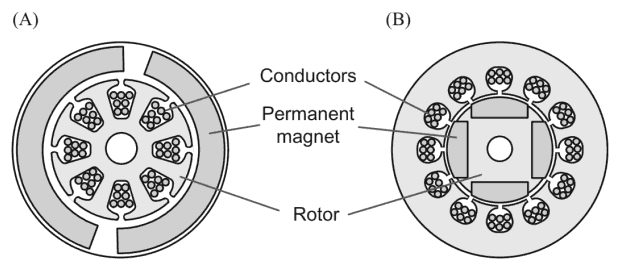
\includegraphics[width=8cm]{imagens/Comparativo.png}
	\caption*{Fonte:\cite{kim2017electric}.}
 \label{Configuração de um motor DC convencional (A) e motor BLDC (B).}
\end{figure}

Amplamente utilizados em uma variedade de aplicações, desde eletrônicos de consumo, como ventiladores e ferramentas elétricas, até aplicações industriais e automotivas. Sua capacidade de fornecer um controle preciso de velocidade e posição, juntamente com uma resposta rápida, faz deles a escolha ideal para sistemas que exigem rendimento energético e alta performance.

Apesar das muitas vantagens, não estão isentos de algumas limitações. A complexidade eletrônica necessária para o controle preciso, o custo inicial potencialmente mais elevado comparado a motores elétricos escovados, a sensibilidade a ambientes de alta temperatura, pois podem gerar a desmagnetização dos imãs permanentes, a exigência de eletrônica de controle especializada, o potencial de ruído eletromagnético (EMI) e a complexidade de manutenção do sistema como um todo são fatores a serem considerados ao escolher essa tecnologia. Cada aplicação específica deve ponderar essas considerações em relação aos benefícios que os BLDC oferecem, como rendimento, durabilidade e controle superior.

São categorizados como síncronos, ou seja, o rotor gira na mesma frequência do campo magnético gerado pelo estator \cite{jahns1984torque}. Também não apresentam o fenômeno de escorregamento que é característico dos motores de indução. Os motores BLDC estão disponíveis em configurações de uma fase, duas fases e três fases, sendo  essa a mais amplamente utilizada, por serem equilibrados em relação a oscilação de torque e custo de construção \cite{hendershot1994design}.

A nomenclatura "Brushless DC" pode gerar uma interpretação equivocada. Embora alimentado por uma fonte de corrente contínua (DC), o motor BLDC é, em sua essência, um motor síncrono de ímãs permanentes (PMSM) \parencite{maquinasEletricasFitzgerald}. A rotação é induzida por campos magnéticos girantes gerados nos enrolamentos do estator, que são alimentados por formas de onda de corrente alternada (AC) sintetizadas por um controlador eletrônico. Portanto, a designação "DC" refere-se à fonte de alimentação externa, e não ao princípio físico de operação interna, que requer uma lógica de controle sofisticada para operar \parencite{ti2013sensorless}.

Nesse contexto, a performance do sistema é governada por parâmetros intrínsecos que descrevem a física da conversão de energia. Duas das mais importantes dessas constantes são a \textbf{constante de torque ($K_T$)} e a \textbf{constante de velocidade ($K_V$)}. Estes parâmetros são a manifestação matemática dos princípios físicos que regem a interação entre os domínios elétrico e mecânico do motor.

\subsection{Fundamentos Físicos da Conversão Eletromecânica}

A operação de um motor elétrico é governada por dois princípios físicos interligados: a Força de Lorentz, que gera o torque, e a Lei da Indução de Faraday, que gera uma força contraeletromotriz.

\subsubsection{A Força de Lorentz e a Condição de Torque Máximo}

A produção de força mecânica em um motor origina-se na Força de Lorentz. Esta lei descreve a força ($\vec{F}$) sobre um condutor de comprimento vetorial ($\vec{L}$) percorrido por uma corrente ($I$) e imerso em um campo magnético ($\vec{B}$). A relação vetorial é:
\begin{equation}
    \vec{F} = I(\vec{L} \times \vec{B})
\end{equation}
A magnitude desta força, $F = I L B \sin(\theta)$, onde $\theta$ é o ângulo entre o condutor e o campo magnético, é maximizada quando $\sin(\theta) = 1$, o que ocorre precisamente quando $\theta = 90^{\circ}$. Esta condição de ortogonalidade é o princípio mais elementar para a máxima conversão de energia.

Em um motor rotativo, o objetivo é o torque, que pode ser entendido como a interação entre o campo magnético gerado pelo estator ($\vec{B}_{\text{estator}}$) e o campo gerado pelos ímãs permanentes do rotor ($\vec{B}_{\text{rotor}}$). O torque eletromagnético ($\vec{T}_{em}$) é o produto vetorial desses dois campos \cite{vas1998vector}:
\begin{equation}
    \vec{T}_{em} \propto \vec{B}_{\text{estator}} \times \vec{B}_{\text{rotor}}
\end{equation}
A magnitude do torque é, portanto, diretamente proporcional ao seno do ângulo elétrico ($\theta_e$) entre os dois vetores de campo. O torque máximo é alcançado quando este ângulo é mantido em 90 graus elétricos. Manter esta condição de ortogonalidade de forma contínua é o objetivo central das estratégias de controle de alto desempenho, como o Controle Orientado por Campo (FOC), pois garante não apenas o torque máximo para uma dada corrente, mas também a máxima eficiência na conversão eletromecânica.

\subsubsection{A Lei de Faraday}
Simultaneamente à produção de torque, um motor em rotação atua como um gerador. A Lei da Indução de Faraday afirma que a variação do fluxo magnético através de uma espira de fio induz uma força eletromotriz (FEM). Em um motor, o movimento dos ímãs do rotor em relação aos enrolamentos do estator induz uma tensão conhecida como \textbf{força contraeletromotriz (FCEM)}, ou \textit{back-EMF}.

De acordo com a Lei de Lenz, a polaridade desta tensão induzida ($e_a$) se opõe diretamente à tensão terminal ($V$) aplicada ao motor \parencite{infineon2011bldc}. A magnitude da FCEM é diretamente proporcional à velocidade angular ($\omega$) do motor, estabelecendo a ligação física entre o movimento mecânico (velocidade) e um fenômeno elétrico (tensão induzida).

\subsection{Modelo Matemático do Motor e a Definição das Constantes}

Os princípios de Lorentz e Faraday são sintetizados em um modelo matemático que descreve a dinâmica do motor.

\textbf{Equação Elétrica (Lei de Kirchhoff):}
\begin{equation}
    V = e_a + I_a R_a + L_a \frac{dI_a}{dt}
\end{equation}
Onde $V$ é a tensão aplicada, $e_a$ é a FCEM de Armadura, $I_a R_a$ é a queda de tensão resistiva de Armadura e $L_a \frac{dI_a}{dt}$ é a queda de tensão indutiva de Armadura \parencite{maquinasEletricasFitzgerald}. Vale ressaltar que Armadura é o termo técnico para o enrolamento em motores elétricos, onde a principal conversão de energia acontece.

\textbf{Equação Mecânica (2ª Lei de Newton para Rotação):}
\begin{equation}
    T_e = T_l + J \frac{d\omega}{dt} + B\omega
\end{equation}
Onde $T_e$ é o torque eletromagnético, $T_l$ é o torque de carga, $J\frac{d\omega}{dt}$ é o torque inercial e $B\omega$ é o torque de atrito viscoso \parencite{maquinasEletricasFitzgerald}.

Dentro deste modelo, as constantes do motor surgem como os fatores de proporcionalidade que conectam os domínios elétrico e mecânico.

\subsection{\texorpdfstring{A constante de Torque $K_T$}{A constante de Torque KT}}
\label{KT}
A constante de torque ($K_T$) define a capacidade de um motor de converter corrente elétrica em torque mecânico. É formalmente definida como a relação linear:
\begin{equation}
    T_e = K_T I_a
\end{equation}
O valor de $K_T$ não é arbitrário, mas determinado pelas características construtivas do motor \parencite{hendershot1994design}:
\begin{itemize}
    \item \textbf{Força do Campo Magnético ($B$):} Ímãs mais fortes (ex: Neodímio) resultam em um $K_T$ maior.
    \item \textbf{Configuração do Enrolamento:} É diretamente proporcional ao número de espiras ($N$) nos enrolamentos.
    \item \textbf{Geometria do Motor:} Dimensões como o comprimento e o raio do estator influenciam diretamente seu valor.
\end{itemize}
Para um dado torque de carga, um motor com $K_T$ maior demandará uma corrente menor, resultando em menores perdas por efeito Joule ($P = I^2 R$) e, portanto, maior eficiência.

\subsection{\texorpdfstring{As constantes de Velocidade $K_V$}{As constantes de Velocidade KV}}
\label{KV}

De forma análoga, a relação entre a FCEM e a velocidade é quantificada por constantes.
\begin{itemize}
    \item \textbf{Constante de FCEM ($K_e$):} É a constante física que relaciona a FCEM gerada ($e_a$) com a velocidade angular do motor ($\omega$):
    \begin{equation}
        e_a = K_e \omega
    \end{equation}
    Assim como $K_T$, $K_e$ (também denotado como $k_b$) depende do projeto físico do motor \parencite{zoltan2012understanding}.

    \item \textbf{Constante de Velocidade ($K_V$):} Muito mais comum em folhas de dados comerciais, $K_V$ é definida como a relação entre a velocidade do motor sem carga e a tensão aplicada, geralmente em unidades de \textbf{RPM/V}. A relação entre $K_V$ e $K_e$ é de simples inversão \parencite{infineon2011bldc}:
    \begin{equation}
        K_V = \frac{1}{K_e}
    \end{equation}
    A FCEM é o mecanismo que limita a velocidade máxima do motor. O motor acelera até que a FCEM ($e_a = K_e \omega$) se aproxime da tensão de alimentação ($V$), ponto no qual a corrente resultante é apenas suficiente para vencer o atrito.
\end{itemize}

\subsection{A Equivalência entre $K_T$ e $K_e$}

Um dos resultados mais notáveis na teoria de motores é a equivalência numérica entre $K_T$ e $K_e$ quando ambas são expressas em unidades do Sistema Internacional (SI): \textbf{Nm/A} para $K_T$ e \textbf{V·s/rad} para $K_e$.
\begin{equation}
    K_T \text{ [Nm/A]} = K_e \text{ [V·s/rad]}
\end{equation}
Esta equivalência não é uma coincidência, mas uma consequência da \textbf{lei da conservação de energia}.

\textbf{Demonstração por Balanço de Potência:}
\begin{enumerate}
    \item A potência elétrica convertida em potência mecânica ($P_{\text{conv}}$) é a parte da potência de entrada que não é perdida como calor nos enrolamentos.
    \
    \item Usando a equação elétrica ($V = e_a + I_a R_a$), substituímos $V$:
    \
    \item A potência mecânica de saída ($P_{\text{mec}}$) é o produto do torque e da velocidade angular:
    \
    \item Pela conservação de energia, $P_{\text{conv}} = P_{\text{mec}}$:
    \
    \item Agora, substituímos as definições de $K_e$ e $K_T$ ($e_a = K_e \omega$ e $T_e = K_T I_a$):
    \
    \item Para qualquer condição de operação não nula, podemos cancelar $\omega$ e $I_a$ de ambos os lados, provando que:
    \begin{equation}
        K_e = K_T
    \end{equation}
\end{enumerate}
Esta prova revela que o mesmo mecanismo de acoplamento eletromagnético que produz torque a partir da corrente (princípio motor, $K_T$) é o que gera tensão a partir do movimento (princípio gerador, $K_e$). Eles são duas manifestações do mesmo fenômeno físico \parencite{zoltan2012understanding, garcia1997modelagem}.

\subsection{Conversão de Unidades}

A elegância teórica é frequentemente obscurecida pelo uso de unidades inconsistentes na prática. A habilidade de converter valores de folhas de dados para o padrão SI é indispensável. A relação prática mais importante é entre $K_T$ e $K_V$:
\begin{equation}
    K_T \text{ [N·m/A]} = \frac{2\pi }{60 \: K_V \text{ [RPM/V]}}
\end{equation}
Esta fórmula é derivada diretamente da equivalência $K_T = K_e = 1/K_V$ após a conversão de RPM para rad/s \parencite{infineon2011bldc}. A tabela abaixo resume as conversões chave.

\begin{table}[h!]
\centering
\caption{Unidades de Constantes de Motor e Fatores de Conversão para o SI}
\label{tab:unidades}

\resizebox{\columnwidth}{!}{

\begin{tabular}{llll}
\toprule
\textbf{Parâmetro} & \textbf{Unidade SI} & \textbf{Unidades Comuns Não-SI} & \textbf{Fórmula de Conversão para SI} \\
\midrule
\textbf{Constante de Torque ($K_T$)} & N·m/A & oz-in/A & 1 oz-in/A = 0.00706155 N·m/A \\
 & & mN·m/A & 1 mN·m/A = 0.001 N·m/A \\
\addlinespace
\textbf{Constante de FCEM ($K_e$)} & V·s/rad & V/krpm & 1 V/krpm = 0.009549 V·s/rad \\
\addlinespace
\textbf{Constante de Velocidade ($K_V$)} & rad/(V·s) & RPM/V & 1 RPM/V = 0.10472 rad/(V·s) \\
\bottomrule
\end{tabular}
}
\caption*{Fonte:Elaborado pelo autor.}
\end{table}

\subsection{A Constante do Motor ($K_m$) como Figura de Mérito}

Uma constante mais fundamental para avaliar a qualidade do projeto de um motor é a \textbf{constante do motor ($K_m$)}:
\begin{equation}
    K_m = \frac{K_T}{\sqrt{R_a}}
\end{equation}
Sua unidade no SI é \textbf{N·m/$\sqrt{\text{W}}$}. $K_m$ representa a capacidade do motor de produzir torque por watt de potência dissipada como calor. Um $K_m$ mais alto indica um motor mais eficiente na conversão de energia. Notavelmente, $K_m$ é invariante a alterações no enrolamento para um mesmo tamanho de carcaça, tornando-se uma excelente figura de mérito para comparar a qualidade de diferentes projetos de motores \parencite{infineon2011bldc}.

\subsection{Influência da Temperatura}

Embora chamadas de "constantes", $K_T$ e $K_e$ são afetadas pela temperatura. O aquecimento do motor causa uma redução na força magnética dos ímãs permanentes. Como ambas as constantes são diretamente proporcionais à densidade de fluxo magnético, um motor operando em alta temperatura produzirá menos torque para a mesma corrente (menor $K_T$) e precisará girar mais rápido para gerar a mesma FCEM (menor $K_e$, consequentemente um $K_V$ ligeiramente maior), resultando em uma performance geral degradada.

\section{Controlador Eletrônico de Velocidade (ESC)} 
 Os controladores eletrônicos de velocidade, são dispositivos eletrônicos que controlam a velocidade e o torque de motores BLDC. São classificados pela sua corrente e tensão máxima de saída. São constituídos dos seguintes componentes básicos: 

 \begin{itemize} 
 \item Circuito de entrada: O circuito de entrada converte a tensão fornecida pela bateria em tensão que pode ser usada pelo circuito de controle utilizando PWM para gerar uma tensão média desejada que será fornecida ao motor. Também pode inverter a sequência de comutação das fases fazendo com que o sentido de rotação também seja invertido. 
 \item Circuito de controle: O circuito de controle é responsável por calcular a corrente que deve ser fornecida às bobinas do motor. Normalmente se utilizam de sinais com características de PWM como sinal de referência para definir a velocidade e sentido de rotação. 
 \item Circuito de saída: O circuito de saída fornece a corrente necessária às bobinas do motor. 
 \end{itemize} 

 Além desses componentes básicos, os ESCs para motor BLDC pode incluir os seguintes recursos, além dos já discutidos anteriormente: 

 \begin{itemize} 
 \item Filtro de ruído: O filtro de ruído é usado para reduzir o ruído elétrico que pode ser gerado pelo motor. 
 \item Proteção térmica: A proteção térmica é usada para proteger o motor de superaquecimento. 
 \item Proteção contra sobrecarga: O ESC pode desligar o motor se ele experimentar correntes superiores às nominais que representam riscos de deterioração das bobinas do motor. 
 \end{itemize} 

  As equações lineares de um motor DC só são diretamente aplicáveis a um motor BLDC devido à ação sofisticada do seu \textbf{Controlador Eletrônico de Velocidade (ESC)}. O ESC realiza a comutação eletrônica, energizando sequencialmente os enrolamentos do estator para criar um campo magnético giratório. Isso força a complexa máquina AC a se comportar como o motor DC idealizado, tornando as constantes $K_T$ e $K_e$ ferramentas de análise e projeto perfeitamente válidas \parencite{hendershot1994design}.

 \subsection{Consequências Práticas da Seleção de $K_V$} 

 A seleção de $K_V$ é uma decisão de projeto crítica que estabelece um compromisso fundamental: 
 \begin{itemize} 
 \item \textbf{Motores de Alto $K_V$:} Possuem menos espiras de fio mais grosso. Resultam em baixo $K_T$, baixa resistência e baixa indutância. Para produzir torque, exigem alta corrente, mas atingem altas velocidades. Ideais para aplicações de alta velocidade e baixo torque, como drones de corrida e fusos de usinagem \parencite{tmotor2019kv}. 
 \item \textbf{Motores de Baixo $K_V$:} Possuem mais espiras de fio mais fino. Resultam em alto $K_T$, alta resistência e alta indutância. Geram alto torque com baixas correntes, sendo mais eficientes para essa finalidade, mas com menor velocidade máxima. Ideais para aplicações de acionamento direto e alto torque, como drones de carga, guinchos e atuadores robóticos \parencite{byod2018kv}. 
 \end{itemize} 

 \subsection{Princípios de Operação} 

  O controlador do motor deve fornecer corrente e tensão adequadas às bobinas do estator do motor, a fim de controlar a velocidade e o torque do motor \cite{jahns1996pulsating}. O circuito básico que realiza esse papel é o de uma ponte inversora trifásica, onde o motor BLDC pode estar conectado em Estrela ou Delta. O controle do circuito de disparo dos transistores do inversor deve ser feito de forma que cada fase do estator seja percorrida por uma corrente com a forma de onda senoidal ou trapezoidal, voltadas respectively para alto rendimento e baixo custo. As formas de onda de cada uma das fases devem estar defasadas entre si, permitindo que o motor gire de forma contínua. 

 \subsubsection{Comutação de Seis Passos} 

 A comutação de seis passos demanda um sincronismo de disparo dos transistores, de modo que sempre dois deles estejam fechados, formando um circuito tal que a cada $60 ^\circ$ elétricos o par de fases percorridas pela corrente se alterne (Figura \ref{Sequência de acionamento para um BLDC trifásico}). Cada transistor permanece em condução durante $120 ^\circ$ elétricos. Vale ressaltar que os eventos de condução e bloqueio, denominados comutações dos transistores, geram variações na corrente e isso é responsável pelas oscilações no torque do motor \cite{kim2017electric}.  

 \begin{figure}[p] 
     \centering 
     \caption{Sequência de acionamento para um BLDC trifásico.} 
     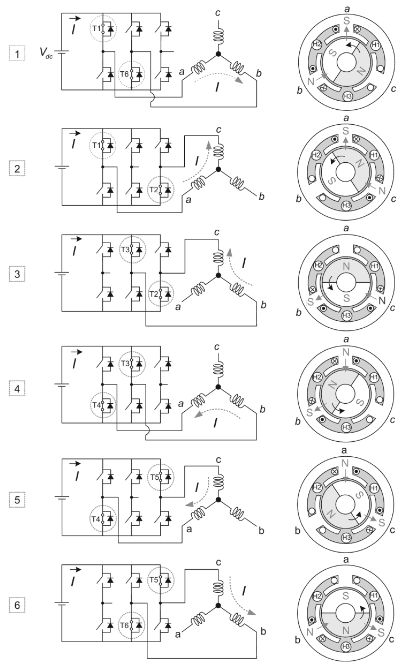
\includegraphics[width=10cm]{imagens/acionamento.png} 
     \caption*{Fonte:\cite{kim2017electric}.} 
  \label{Sequência de acionamento para um BLDC trifásico} 
 \end{figure} 

Esse algoritmo de acionamento dos transistores, também chamado de Controle Trapezoidal, é a base para o funcionamento do motor BLDC. Embora seja possível operá-lo em malha aberta (sequência fixa), esta abordagem é ineficiente e propensa a perda de sincronismo sob variações de carga. Portanto, neste trabalho, adota-se o **Controle de Malha Fechada \textit{Sensorless}**.

Nesta topologia, a sequência de comutação não é fixa no tempo, mas sincronizada dinamicamente com a posição do rotor. A detecção da posição é realizada monitorando-se a Força Contraeletromotriz (FCEM) na fase não energizada. Assim, o microcontrolador detecta o momento exato em que o rotor cruzou uma posição angular específica e dispara a próxima comutação, garantindo que o ângulo entre os campos magnéticos permaneça próximo de $90^\circ$ elétricos (torque máximo).

 Quando a aplicação necessita que o motor possua apenas uma velocidade, a fonte de alimentação de tensão fixa é suficiente. Para casos onde é necessário variar a velocidade do motor, a técnica de Modulação por Largura de Pulso (PWM) é normalmente empregada. Um ESC, por exemplo, utiliza PWM para ajustar a tensão média aplicada ao motor, controlando assim sua velocidade. Essa técnica, no entanto, pode demandar a utilização de controladores que comparem a velocidade desejada com a medida no rotor para um controle preciso. 

 \subsubsection{Análise da Ondulação de Torque (Torque Ripple)}
A principal desvantagem intrínseca à comutação forçada de seis passos (malha aberta) é a geração de uma ondulação de torque (\textit{torque ripple}), que se manifesta como pulsações no torque de saída do motor \cite{jahns1984, ali2017implementation}. Essas pulsações podem causar oscilações na velocidade, ruído acústico e vibrações mecânicas, sendo particularmente prejudiciais em aplicações que exigem alta precisão de movimento \cite{jahns1996pulsating}. A frequência desta ondulação é seis vezes a frequência elétrica fundamental do motor, correspondendo a uma pulsação a cada evento de comutação \cite{jahns1984}. Conforme analisado em trabalhos seminais como os de Jahns (1984) e Hendershot \& Miller (1994), este fenômeno é consequência de dois fatores principais \cite{kim2017, hendershot1994design}.

\begin{enumerate}
    \item \textbf{Incompatibilidade de Formas de Onda:} O modelo ideal do controle trapezoidal assume uma forma de onda de corrente perfeitamente retangular e uma FCEM perfeitamente trapezoidal. Na prática, a FCEM dos motores reais raramente é um trapézio ideal, e a corrente injetada não é perfeitamente retangular. Qualquer desalinhamento ou incompatibilidade entre a forma de onda da corrente e a da FCEM resulta em variações no torque produzido, conforme a equação $T_{e} = (e_{a}i_{a} + e_{b}i_{b} + e_{c}i_{c}) / \omega$ \cite{hendershot1994design}.

    \item \textbf{Transientes de Comutação:} A causa mais significativa da ondulação de torque é o próprio processo de comutação. Devido à indutância presente nos enrolamentos do motor, a corrente não pode variar instantaneamente. Quando o controlador comuta de um passo para o outro (por exemplo, de A-B para A-C), há um período de tempo finito durante o qual a corrente na fase que está sendo desligada (fase B) decai, e a corrente na fase que está sendo ligada (fase C) aumenta \cite{jahns1996pulsating, joice2013compensation}. Durante este intervalo de comutação, o torque eletromagnético total produzido pelo motor não é constante. A taxa de variação da corrente na fase de entrada e na de saída não é necessariamente simétrica, resultando em um mergulho ou pico de torque a cada $60^{\circ}$ elétricos \cite{choi1998commutation, chen2019commutation}.
\end{enumerate}

A ondulação de torque não é apenas um efeito colateral indesejado; é a manifestação mecânica de uma conversão de energia eletromecânica periodicamente ineficiente. O objetivo do motor é converter potência elétrica em potência mecânica (torque vezes velocidade) de forma contínua e suave. Durante os intervalos de comutação, o vetor de corrente do estator está em transição entre duas posições estáveis. Neste período, o alinhamento entre o campo magnético do estator e o campo magnético do rotor desvia-se momentaneamente da orientação ótima de $90^{\circ}$ elétricos necessária para a produção máxima de torque. Consequentemente, para uma mesma magnitude de corrente de entrada, o torque de saída é reduzido, representando uma queda transitória na eficiência da conversão de energia. A ondulação de torque observada é, portanto, o resultado direto desses intervalos de conversão sub-ótima, inerentes à natureza discreta do chaveamento de seis passos.

 \subsubsection{Modulação por Largura de Pulso} 

 Fontes de tensão fixa, como baterias, são as mais acessíveis do mercado. A partir delas, é possível gerar uma tensão média de alimentação variável utilizando uma técnica conhecida como PWM (Modulação por Largura de Pulso), permitindo o controle de velocidade de um BLDC. Para isso, utiliza-se um circuito simples capaz de transformar a tensão contínua em uma onda quadrada de frequência fixa e amplitude igual à tensão da fonte de alimentação. A própria ponte trifásica pode ajustar a largura dos pulsos, fazendo com que a tensão média entregue à ponte inversora seja proporcional à velocidade desejada (Figura \ref{Modulação por largura de pulso utilizando uma fonte de 100V}). 

 \begin{figure}[h] 
     \centering 
     \caption{Modulação por largura de pulso utilizando uma fonte de $100V$.} 
     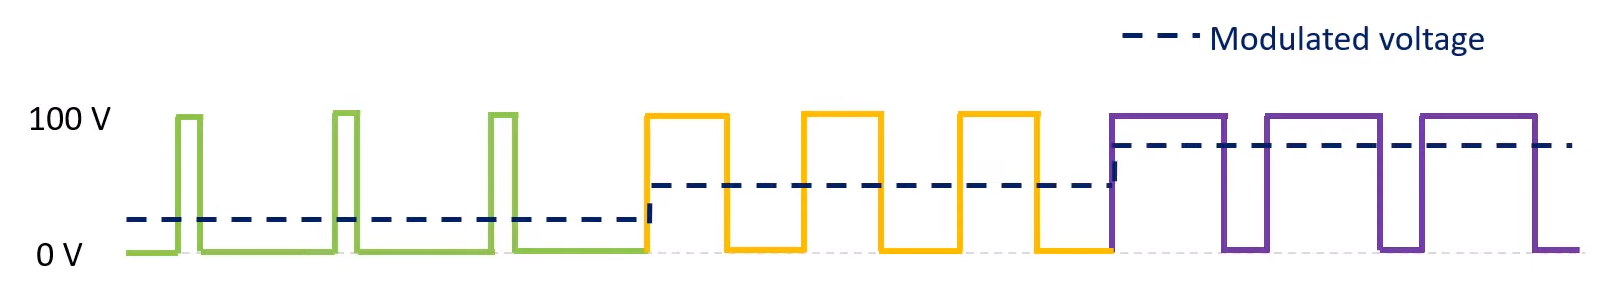
\includegraphics[width=13cm]{imagens/PWM.png} 
     \caption*{Fonte:\cite{matlabBLDC}.} 
  \label{Modulação por largura de pulso utilizando uma fonte de 100V} 
 \end{figure} 

 \subsection{Estratégia de Partida em Malha Aberta para Operação \textit{Sensorless}}

A implementação de um controle \textit{sensorless} eficaz depende da capacidade do controlador de estimar a posição do rotor a partir de grandezas elétricas, mais comumente a FCEM. Contudo, esta abordagem apresenta um desafio fundamental: em repouso (velocidade zero), não há movimento relativo entre os ímãs do rotor e os enrolamentos do estator, e, portanto, nenhuma FCEM é gerada \cite{ti2013sensorless, nxp2023sensorless}. Nesta condição "cega", o controlador não possui informações sobre a posição angular do rotor, tornando impossível determinar qual par de fases deve ser energizado para iniciar a rotação na direção desejada. Para superar essa limitação, é necessária uma rotina de partida especializada, operando em malha aberta, que força o motor a girar até que uma velocidade suficiente seja atingida para que a FCEM se torne detectável e o controle em malha fechada possa assumir. Este procedimento é universalmente dividido em duas fases sequenciais: alinhamento e comutação forçada.

\subsubsection{Alinhamento do Rotor}

O primeiro passo para uma partida confiável é estabelecer uma posição inicial conhecida para o rotor. A fase de alinhamento realiza isso ao energizar um conjunto específico de enrolamentos do estator com uma corrente contínua (DC) por um período de tempo pré-determinado \cite{ti2022minimizing, nxp2023sensorless}. Por exemplo, o controlador pode aplicar uma tensão positiva à fase C e conectar as fases A e B ao terra \cite{ti2022minimizing}. Esta ação cria um campo magnético estático e fixo no estator. Os ímãs permanentes do rotor, livres para girar, irão se alinhar com este campo para minimizar a relutância magnética do circuito, de forma análoga a uma agulha de bússola se alinhando com o campo magnético terrestre. Ao final deste processo, o rotor estará travado em uma posição angular conhecida e previsível. Os parâmetros críticos que governam esta fase são a duração do alinhamento e a magnitude da corrente de alinhamento \cite{ti2022minimizing}.

 A fase de alinhamento funciona como uma etapa de otimização pré-torque, o seu objetivo primordial é condicionar o sistema para que o primeiro passo de comutação dinâmica gere o máximo torque possível. O maior desafio ao iniciar um motor a partir do repouso é vencer a inércia da carga e o atrito estático, o que exige um impulso de torque inicial elevado. A teoria de motores elétricos, conforme estabelecido na Seção 1.1.1, dita que o torque é maximizado quando o campo magnético do estator está orientado a $90^{\circ}$ elétricos em relação ao campo do rotor. O algoritmo de controle é projetado sabendo a posição final do rotor após o alinhamento. Assim, a primeira combinação de fases a ser energizada na fase seguinte (rampa de aceleração) é escolhida para criar um novo vetor de campo magnético do estator que esteja precisamente na orientação ótima em relação à posição agora conhecida do rotor. Isso garante que o primeiro passo dinâmico produza um torque potente e eficaz, "chutando" o rotor para o movimento e superando as resistências iniciais. Uma duração de alinhamento insuficiente ou uma corrente muito baixa pode resultar em um alinhamento incompleto, levando a um torque inicial fraco e, consequentemente, a uma falha na partida \cite{ti2022minimizing, jones2025failures}.

\subsubsection{Comutação Forçada (Rampa de Aceleração)}

Com o rotor devidamente alinhado, o controlador inicia a fase de comutação forçada. Nesta etapa, o sistema opera em malha aberta, comutando as fases em uma sequência predefinida, sem qualquer realimentação da posição do rotor \cite{nxp2023sensorless}. A frequência de comutação não é aplicada abruptamente; em vez disso, ela é aumentada gradualmente a partir de um valor inicial baixo, seguindo um perfil de aceleração pré-programado, conhecido como "curva de partida em malha aberta" (\textit{open-loop starting curve}) \cite{ti2022minimizing}. Esta rampa de aceleração é definida por coeficientes pré-definidos \cite{ti2022minimizing}.

Durante esta fase, o controlador essencialmente comanda a rotação do campo magnético do estator e "assume" que o rotor, devido à sua inércia e ao torque gerado, conseguirá acompanhar este campo giratório. O processo continua, com a frequência de comutação aumentando progressivamente, até que a velocidade de rotação do motor seja alta o suficiente (tipicamente em torno de $5\%$ da velocidade nominal) para que a FCEM gerada nos enrolamentos atinja uma amplitude que possa ser medida de forma confiável \cite{ti2022minimizing, nxp2023sensorless}. Neste ponto, o sistema realiza a transição (\textit{handoff}) do controle em malha aberta para um modo de controle em malha fechada (por exemplo, baseado na detecção de cruzamento por zero da FCEM), que é mais eficiente e robusto para a operação contínua.

\subsection{Desafios e Limitações da Partida Forçada}

A estratégia de partida em malha aberta não é isenta de desafios e limitações significativas. A sua natureza "cega" a torna vulnerável a variações de carga e a parâmetros não ideais do sistema.

\subsubsection{Análise do Fenômeno de Perda de Sincronismo (Stall)}

O risco mais proeminente do controle em malha aberta é a perda de sincronismo, comumente conhecida como \textit{stall} ou perda de passo. Este fenômeno ocorre quando a aceleração real do rotor não consegue acompanhar a velocidade de rotação do campo magnético do estator imposta pelo controlador. Se o torque de carga aplicado ao eixo do motor, somado à sua própria inércia, for maior que o torque eletromagnético que o motor consegue produzir em um determinado passo, o rotor "perderá o passo" e ficará para trás \cite{nxp2023sensorless}. Isso pode ser causado por uma carga inicial muito elevada ou por uma rampa de aceleração excessivamente agressiva, que aumenta a frequência de comutação mais rápido do que o rotor consegue acelerar \cite{ti2022minimizing}.

Uma vez que o sincronismo é perdido, o alinhamento entre os campos do rotor e do estator se torna desfavorável, e a produção de torque efetivo colapsa. O resultado é um movimento errático, vibrações intensas, ruído audível e, frequentemente, a parada completa do motor, enquanto o controlador continua a injetar corrente nos enrolamentos de forma ineficaz. Este estado pode levar a picos de corrente perigosos para a eletrônica de potência. Por essa razão, o controle em malha aberta é inadequado para aplicações com cargas variáveis ou que exigem alto torque de partida.

\subsubsection{Outros Efeitos Adversos}

Além do risco de perda de passo, a partida forçada apresenta outras desvantagens:

\begin{itemize}
    \item \textbf{Picos de Corrente:} No início da partida, a velocidade do motor é baixa ou nula, o que significa que a FCEM, que normalmente se opõe à tensão de alimentação e limita a corrente, também é baixa ou inexistente. Sem essa oposição, a corrente que flui para os enrolamentos é limitada apenas pela resistência ôhmica e pela tensão aplicada, podendo atingir valores muito elevados se não for cuidadosamente controlada pelo \textit{duty cycle} do PWM. Estes picos de corrente podem estressar a bateria e os componentes da ponte inversora.
    \item \textbf{Vibração e Ineficiência:} Como o controle é feito "às cegas", o alinhamento entre o campo do estator e o rotor durante a rampa de aceleração nunca é perfeito. Este desalinhamento constante é a fonte da ondulação de torque discutida anteriormente, que se manifesta como vibração mecânica e resulta em uma operação ineficiente, onde uma parte da energia elétrica consumida é dissipada em vez de ser convertida em torque útil.
\end{itemize}

É fundamental reiterar que a partida forçada em malha aberta é uma fase transitória e um meio para um fim. É uma estratégia de \textit{bootstrap} projetada exclusivamente para levar o motor de um estado de repouso para uma velocidade operacional mínima, onde métodos de controle em malha fechada, mais eficientes, precisos e robustos, podem ser ativados para a operação contínua do sistema \cite{ti2022minimizing, nxp2023sensorless}.

\section{Aspectos de Eletrônica de Potência}

A implementação física do inversor exige a compreensão de componentes e técnicas que viabilizam a comutação em alta frequência e corrente.

\subsection{O MOSFET de Potência e Perdas}
O MOSFET (\textit{Metal-Oxide-Semiconductor Field-Effect Transistor}) é o dispositivo de chaveamento predominante em aplicações de baixa e média tensão devido à sua alta velocidade de comutação e facilidade de acionamento \cite{rashid2014power}. Em um inversor para controle de motores, o MOSFET não atua na região linear (amplificação), mas alterna entre os estados de corte (chave aberta) e saturação (chave fechada).

A eficiência do inversor é limitada por dois mecanismos principais de perda no MOSFET \cite{kim2017electric}:
\begin{itemize}
    \item \textbf{Perdas por Condução ($P_{cond}$):} Quando o transistor está ligado, ele apresenta uma resistência interna residual entre dreno e fonte, denominada $R_{DS(on)}$. A potência dissipada é dada por $P_{cond} = I_{D}^2 \cdot R_{DS(on)}$. Componentes modernos buscam minimizar o $R_{DS(on)}$ para reduzir o aquecimento.
    \item \textbf{Perdas por Comutação ($P_{sw}$):} Ocorrem durante a transição entre ligado e desligado. Como a tensão e a corrente não variam instantaneamente, há um breve período em que ambas são não-nulas, gerando um pico de potência dissipada. Esta perda é diretamente proporcional à frequência de chaveamento ($f_{sw}$) e à carga total de gate ($Q_g$) que o driver deve fornecer \cite{rashid2014power}.
\end{itemize}

\subsection{O Barramento DC e a Indutância Parasita}

Em inversores de fonte de tensão (VSI) que operam com altas frequências de chaveamento, a impedância da fonte de alimentação não pode ser considerada ideal. Os cabos de conexão entre a bateria e o inversor introduzem uma indutância parasita ($L_{par}$) significativa no circuito. Durante a comutação dos transistores, a rápida variação de corrente ($di/dt$) interage com essa indutância, gerando picos de tensão ($V_{spike}$) de acordo com a lei de Faraday-Lenz:

\begin{equation}
    V_{spike} = L_{par} \cdot \frac{di}{dt}
\end{equation}

Se não mitigados, esses picos podem superar a tensão de ruptura dos semicondutores, causando falhas catastróficas. Para solucionar esse problema, utiliza-se um banco de capacitores no barramento DC (\textit{DC Link}), posicionado fisicamente próximo aos interruptores. Este banco atua como uma fonte de tensão de baixa impedância local, fornecendo a corrente pulsada exigida pelo inversor e absorvendo a energia regenerada, além de filtrar a componente alternada (ripple) da corrente \cite{rashid2014power}.

Embora o cálculo analítico da capacitância mínima ($C_{min}$) seja classicamente derivado da máxima variação de tensão admissível ($\Delta V$) no barramento, conforme a Equação \ref{eq:cap_calc}:

\begin{equation}
    C_{min} = \frac{I_{peak} \cdot D \cdot (1-D)}{f_{sw} \cdot \Delta V}
    \label{eq:cap_calc}
\end{equation}

\noindent onde $f_{sw}$ é a frequência de chaveamento e $D$ é o ciclo de trabalho (\textit{Duty Cycle}) do inversor. Observa-se que o esforço máximo sobre o capacitor ocorre quando $D=0,5$, ponto em que o produto $D(1-D)$ é máximo.

Entretanto, em aplicações de baixa tensão e alta corrente (como em VANTs), o fator limitante do projeto não é apenas a armazenagem de carga ($C_{min}$), mas sim a capacidade de condução de corrente de ripple ($I_{Ripple,RMS}$) e a dissipação térmica. Capacitores eletrolíticos comerciais apresentam uma correlação inversa entre capacitância nominal e Resistência Série Equivalente (ESR).

Consequentemente, adota-se na prática de engenharia o sobredimensionamento do valor de capacitância (regras empíricas da ordem de $10\mu F$ a $20\mu F$ por Ampere de corrente de fase). Esta abordagem visa, primariamente, reduzir a ESR total do banco de capacitores através da associação paralela e do uso de encapsulamentos maiores, garantindo que a corrente eficaz drenada pelo inversor não exceda o \textit{Ripple Current Rating} dos componentes, prevenindo a degradação dielétrica prematura por superaquecimento \cite{rashid2014power}.

\subsection{Técnica de \textit{Bootstrap} para Acionamento \textit{High-Side}}
Em uma ponte inversora trifásica, os transistores do "lado alto" (\textit{High-Side}) têm seus drenos conectados ao barramento positivo ($V_{CC}$) e suas fontes conectadas às fases do motor. Para ligar um MOSFET Canal-N nesta posição, a tensão no \textit{gate} deve ser superior à tensão da fonte ($V_{GS} > V_{th}$). Contudo, quando o transistor liga, a tensão da fonte sobe para aproximadamente $V_{CC}$, exigindo que a tensão do \textit{gate} seja elevada para $V_{CC} + V_{drv}$.

A técnica de \textit{Bootstrap} é a solução mais comum e econômica para gerar essa tensão flutuante. Ela utiliza um capacitor ($C_{boot}$) e um diodo ($D_{boot}$). O princípio de operação é cíclico:
\begin{enumerate}
    \item Quando o transistor do "lado baixo" (\textit{Low-Side}) está ligado, o terminal da fase é aterrado. O capacitor $C_{boot}$ é então carregado através do diodo pela fonte de alimentação auxiliar ($V_{drv}$).
    \item Quando o \textit{Low-Side} desliga e o \textit{High-Side} precisa ser acionado, a carga armazenada em $C_{boot}$ atua como uma "bateria flutuante", fornecendo a corrente necessária para carregar o \textit{gate} do transistor superior.
\end{enumerate}

\textbf{Limitação Importante:} O circuito de \textit{Bootstrap} não permite operação com ciclo de trabalho (\textit{duty cycle}) de 100\% indefinidamente. O transistor \textit{Low-Side} deve ser ligado periodicamente para recarregar o capacitor. Se o capacitor descarregar por falta de comutação, a tensão $V_{GS}$ cai, podendo levar o MOSFET superior a operar na região linear e falhar por superaquecimento.

\subsubsection{Dimensionamento do Capacitor de Bootstrap}

O capacitor de \textit{bootstrap} ($C_{boot}$), embora fisicamente conectado ao circuito do driver, tem como função primária atuar como um reservatório de energia flutuante para alimentar a porta (\textit{gate}) do MOSFET superior \cite{infineonAN978}. O driver atua apenas como a chave de transferência, drenando carga de $C_{boot}$ e injetando-a na capacitância de entrada do MOSFET para promover sua saturação.

Consequentemente, o dimensionamento deste capacitor depende intrinsecamente da quantidade de carga que o MOSFET exige para ligar, parâmetro conhecido como Carga Total de Gate ($Q_g$). A carga total ($Q_{tot}$) demandada do capacitor a cada ciclo de comutação é composta pela carga do MOSFET somada às perdas internas do driver \cite{infineonAN978}:

\begin{equation}
    Q_{tot} = \underbrace{Q_g}_{\text{Carga do MOSFET}} + \underbrace{(I_{qbs} + I_{leak}) \cdot T_{on}}_{\text{Consumo do Driver e Fugas}}
\end{equation}

\noindent onde $I_{qbs}$ é a corrente quiescente do estágio de alta do driver e $I_{leak}$ representa as correntes de fuga. Como $Q_g$ é tipicamente muito maior que o consumo do driver em frequências usuais, ele é o fator determinante no dimensionamento. Para garantir que a tensão no capacitor não sofra uma queda brusca ($\Delta V_{boot}$) ao transferir essa carga para o MOSFET o que poderia reduzir a tensão $V_{GS}$ abaixo do nível seguro de saturação, a capacitância mínima é calculada como \cite{infineonAN978}:

\begin{equation}
    C_{boot} \geq \frac{Q_{tot}}{\Delta V_{boot}}
\end{equation}

Na prática de engenharia, para assegurar robustez contra transitórios e variações de temperatura, adota-se um capacitor capaz de armazenar pelo menos 15 vezes a carga do gate do MOSFET ($Q_g$), garantindo uma fonte de tensão rígida para o driver \cite{adamsDT98}.

\section{Estado da Arte em Algoritmos de Controle e Estimação}
\label{sec:estado_da_arte}

Embora a técnica de comutação trapezoidal com detecção de cruzamento por zero (ZCD) seja robusta e amplamente utilizada, o desenvolvimento de microcontroladores de alto desempenho e FPGAs permitiu a implementação de estratégias de controle mais sofisticadas. Estas técnicas visam superar as limitações do ZCD, principalmente em baixas velocidades e no controle de torque.

\subsection{Métodos Baseados em Força Contraeletromotriz (FCEM)}
Esta categoria, na qual se insere a técnica utilizada neste trabalho, fundamenta-se na proporcionalidade entre a tensão induzida e a velocidade angular do rotor.
\begin{itemize}
    \item \textbf{Detecção de Cruzamento por Zero (ZCD):} Monitora a tensão na fase não energizada para determinar os instantes de comutação. É simples e eficaz para médias e altas rotações.
    \item \textbf{Integração da FCEM:} Em vez de buscar apenas o zero, integra-se a área sob a curva da tensão induzida. Isso oferece maior imunidade a ruídos de PWM (ruído de comutação), pois a integração atua como um filtro natural.
    \item \textbf{Limitação e Solução:} A principal dificuldade é a inexistência de sinal em velocidade zero ou muito baixa. A solução padrão da indústria é a "Comutação Forçada" (\textit{Sensorless Trapezoidal Control}), onde aplica-se uma sequência cega inicial para arrancar o motor até que a FCEM seja detectável.
\end{itemize}

\subsection{Controle Orientado de Campo (FOC) e Observadores}
O Controle Orientado de Campo (\textit{Field-Oriented Control} - FOC) representa o padrão de alto desempenho. Diferente do controle trapezoidal que aciona o motor em passos discretos, o FOC controla as correntes do estator para manter o vetor de campo magnético sempre ortogonal ao rotor (90 graus), maximizando o torque por ampere e reduzindo a ondulação de torque. Para operação sem sensores (\textit{sensorless}), utilizam-se observadores matemáticos:

\begin{itemize}
    \item \textbf{Observadores de Estado (Luenberger):} Utilizam as equações diferenciais do motor para estimar a corrente e a FCEM. A diferença entre a corrente estimada e a medida (erro) é usada para corrigir a estimativa da posição do rotor em tempo real.
    \item \textbf{Filtro de Kalman Estendido (EKF):} Uma abordagem estocástica que considera as incertezas do modelo e o ruído das medições. O EKF prediz o estado futuro do sistema e corrige a predição com base nas medições atuais, sendo extremamente robusto em ambientes ruidosos, embora exija alto poder computacional.
    \item \textbf{Observadores Adaptativos:} Ajustam dinamicamente os parâmetros do modelo (como resistência ou fluxo) durante a operação, compensando variações térmicas que poderiam degradar a precisão da estimativa.
\end{itemize}

\subsection{Técnicas Baseadas em Análise de Sinais e Harmônicos}
Existem métodos que exploram as não-linearidades e características construtivas do motor para inferir a posição, úteis especialmente em baixa velocidade onde a FCEM é nula.
\begin{itemize}
    \item \textbf{Detecção de Ondulação de Corrente (\textit{Current Ripple}):} A interação entre os polos do rotor e as ranhuras do estator gera pequenas ondulações na corrente. Algoritmos de processamento de sinal podem contar essas ondulações para estimar a velocidade e posição.
    \item \textbf{Método de Injeção de Alta Frequência:} Aplica-se um sinal de tensão de alta frequência e baixa amplitude. Devido à saliência magnética do rotor ($L_d \neq L_q$), a resposta de corrente varia conforme a posição angular, permitindo detectar a posição mesmo com o motor parado.
\end{itemize}

\section{Parâmetros Críticos para Modelagem Dinâmica}
\label{sec:parametros_modelagem}

A implementação de algoritmos avançados, como o FOC e os Observadores de Estado, exige um conhecimento preciso dos parâmetros intrínsecos do motor. A precisão do modelo matemático — e consequentemente a qualidade do controle — depende diretamente da caracterização das seguintes grandezas:

\begin{description}
    \item[Resistência de Estator ($R_s$):] Determina a queda de tensão ôhmica nos enrolamentos. Erros na identificação de $R_s$ causam desvios na estimativa de fluxo em baixas velocidades.
    
    \item[Indutância de Estator ($L_s, L_d, L_q$):] Fundamental para determinar a resposta dinâmica da corrente. Em motores de ímãs interiores (IPM), a diferença entre a indutância de eixo direto ($L_d$) e em quadratura ($L_q$) é o que permite o torque de relutância e a detecção de posição por injeção de sinal.
    
    \item[Fluxo do Rotor ($\lambda_m$):] Representa o fluxo magnético gerado pelos ímãs permanentes. É crucial para o cálculo do torque eletromagnético ($T_e$) e da constante de FCEM ($K_e$). Variações de temperatura podem alterar $\lambda_m$ (desmagnetização temporária), afetando a constante $K_T$ do motor.
    
    \item[Momento de Inércia ($J$) e Atrito ($B$):] Parâmetros mecânicos que ditam a resposta de velocidade do sistema. O conhecimento de $J$ é vital para o projeto das malhas de controle de velocidade, influenciando os ganhos $K_p$ e $K_i$ do controlador PID.
    
    \item[Número de Polos ($P$):] Define a relação entre a frequência elétrica e a velocidade mecânica. Um erro neste parâmetro inviabiliza qualquer algoritmo de estimação de velocidade.
\end{description}

O levantamento desses parâmetros geralmente requer equipamentos de precisão ou rotinas de auto-comissionamento implementadas no próprio inversor, destacando a complexidade superior dessas técnicas em comparação ao método trapezoidal via ZCD adotado neste projeto.

 \pagebreak 

 \section{Vantagens e Desvantagens no uso de motores BLDC} 
 Os motores sem escovas, ou BLDC, apresentam diversas vantagens que contribuem para seu destaque em várias aplicações. O rendimento é uma característica proeminente, uma vez que convertem mais eficientemente a energia elétrica em torque quando comparados aos motores com escovas. Isso implica em uma demanda menor de energia para gerar a mesma quantidade de torque, resultando em um melhor desempenho global. A durabilidade é significativamente aprimorada, visto que a vida útil estendida desses motores está relacionada à ausência das escovas, componentes propensos a desgaste em motores convencionais. 

 Os motores de indução trifásicos (MIT) são concorrentes diretos dos motores BLDC, sendo que ambos são amplamente utilizados em diversas aplicações, cada uma com suas características distintas e vantagens específicas. Os motores de indução trifásicos são conhecidos pela sua confiabilidade, simplicidade de construção e custo relativamente baixo, quando comparado aos BLDC, utilizando os princípios da indução eletromagnética para gerar o torque e velocidade necessários para a aplicação. Embora tenham menor custo de produção quando comparados com os motores BLDC e podem ser controlados utilizando os mesmos protocolos, os MITs tendem a ter uma densidade de potência e torque menor em comparação com os motores BLDC, principalmente em baixas velocidades, o que pode ser uma consideração importante em aplicações que requerem alta potência em um espaço limitado. No entanto, os MITs apresentam melhor rendimento em operações de baixo torque, o que pode ser relevante em aplicações de mobilidade, como em veículos elétricos. 

 Os motores BLDC são conhecidos por seu rendimento energético superior, controle preciso de velocidade e torque, além de uma vida útil mais longa devido à ausência de escovas mecânicas \cite{gieras2009permanent}. Embora os BLDCs tenham um custo inicial mais elevado em comparação com os MITs, eles oferecem uma operação mais eficiente, especialmente em condições de carga variável e velocidade ajustável. 

 Em resumo, os motores sem escovas oferecem um conjunto de vantagens notáveis, incluindo rendimento aprimorado, operação mais silenciosa, maior durabilidade e menor necessidade de manutenção. Contudo, esses benefícios vêm com um custo inicial mais elevado e a exigência de um controlador de velocidade, o que pode tornar sua implementação menos acessível em certos contextos. A escolha entre motores com escovas e sem escovas dependerá das prioridades específicas de uma aplicação, considerando tanto os benefícios quanto as limitações de cada tecnologia. 

 \pagebreak 

 \section{Aplicações} 
 Os motores BLDC são amplamente utilizados em diversas aplicações devido às suas características únicas, como elevado rendimento, alta densidade de potência, baixo ruído, baixa manutenção e longa vida útil. Esses motores são preferidos em aplicações que necessitam de controle preciso de torque com oscilações inferiores em comparação com outros motores. 

 Uma das principais aplicações dos motores BLDC é em veículos elétricos, como carros, motocicletas, bicicletas e \textit{scooters} \cite{chau2007emerging}. Com o aumento da demanda por veículos elétricos, espera-se que os motores com tecnologia derivada do BLDC desempenhem um papel vital na indústria automotiva. Esses motores são usados para acionar o sistema de propulsão do veículo, fornecendo torque e potência para as rodas. Eles são preferidos em veículos elétricos devido à seu alta rendimento, baixo ruído e baixa manutenção. Essas motores são usados em aplicações que exigem alta precisão, controle de velocidade e torque, e baixo ruído.

